\lstinputlisting[language=bash,basicstyle=\small]{python_codes/fieldstone_95/keywords}

\begin{center}
Code at \url{https://github.com/cedrict/fieldstone/tree/master/python_codes/fieldstone_95}
\end{center}

\par\noindent\rule{\textwidth}{0.4pt}

%%%%%%%%%%%%%%%%%%%%%%%%%%%%%%%%%%%%%%%%%%%%%%%%%%%%%%%%%%%%%%%%%%%%%%%%%%%%%%%%%%%%%%%%

This stone tackles the Rayleigh-Taylor instability problem of van Keken \etal \cite{vaks97}. 
It builds on Stone 93 as it relies on triangular elements (the MINI element(see Section~\ref{pair:mini}), 
the Taylor-Hood $P_2\times P_1$ element (see Section~\ref{ss:p2p1}), 
and the Crouzeix-Raviart element (see Section~\ref{sec:crouzeix-raviart})) and Delaunay meshes
generated by the Triangle code \cite{shew14}.  

However, this code does implements mesh adaptation and the python code then calls the Triangle mesher code
at every timestep (the remeshing cost is negligible).
I unfortunately cannot prevent Triangle from adding nodes in between the interface nodes, thereby 
ruining the numbering and the flagging of these nodes. I have therefore implemented a refinement 
process which add nodes on the interface when two consecutive nodes are getting too far apart (which 
would have been necessary because of the shear stretching of the interface). 

\begin{center}
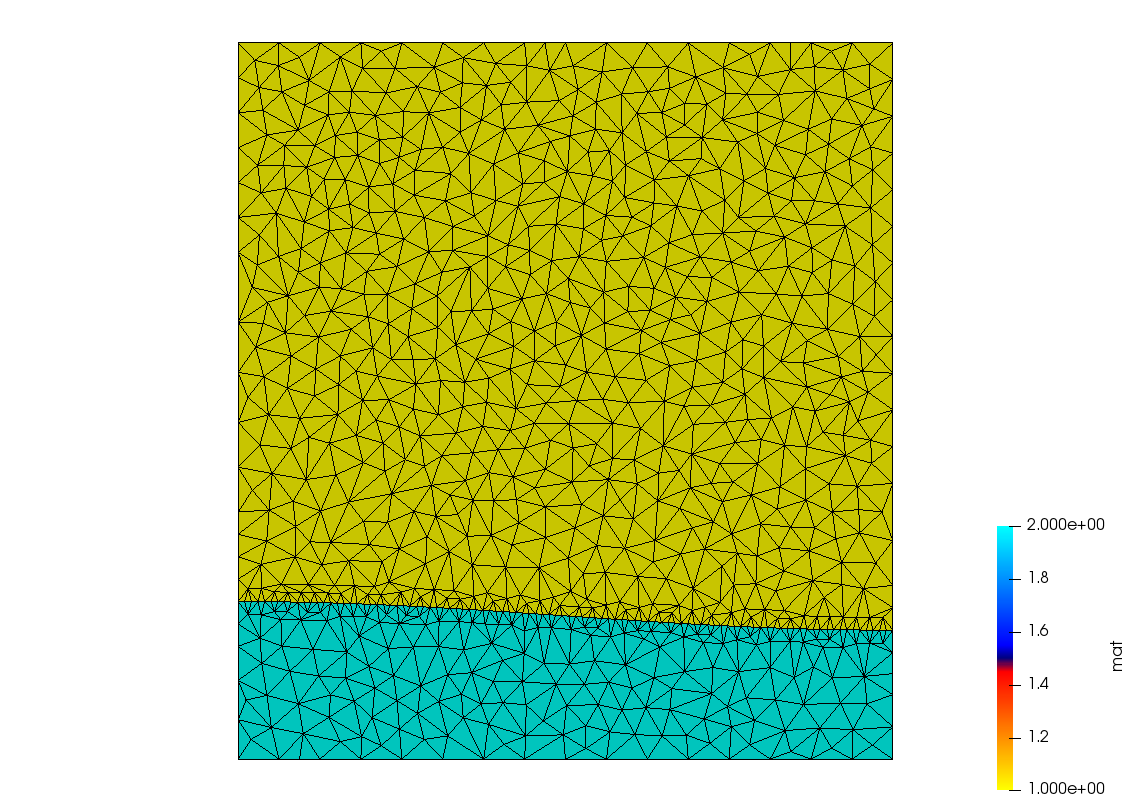
\includegraphics[width=5.5cm]{python_codes/fieldstone_95/init/mat}
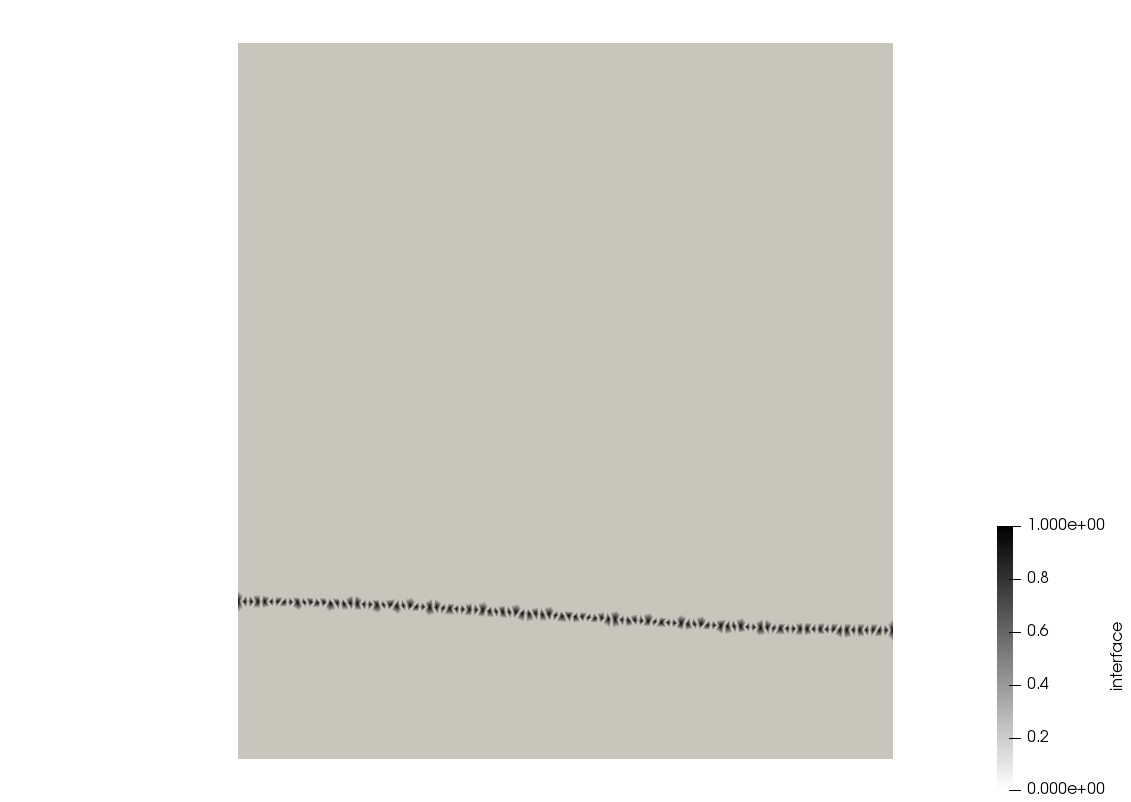
\includegraphics[width=5.5cm]{python_codes/fieldstone_95/init/interface}
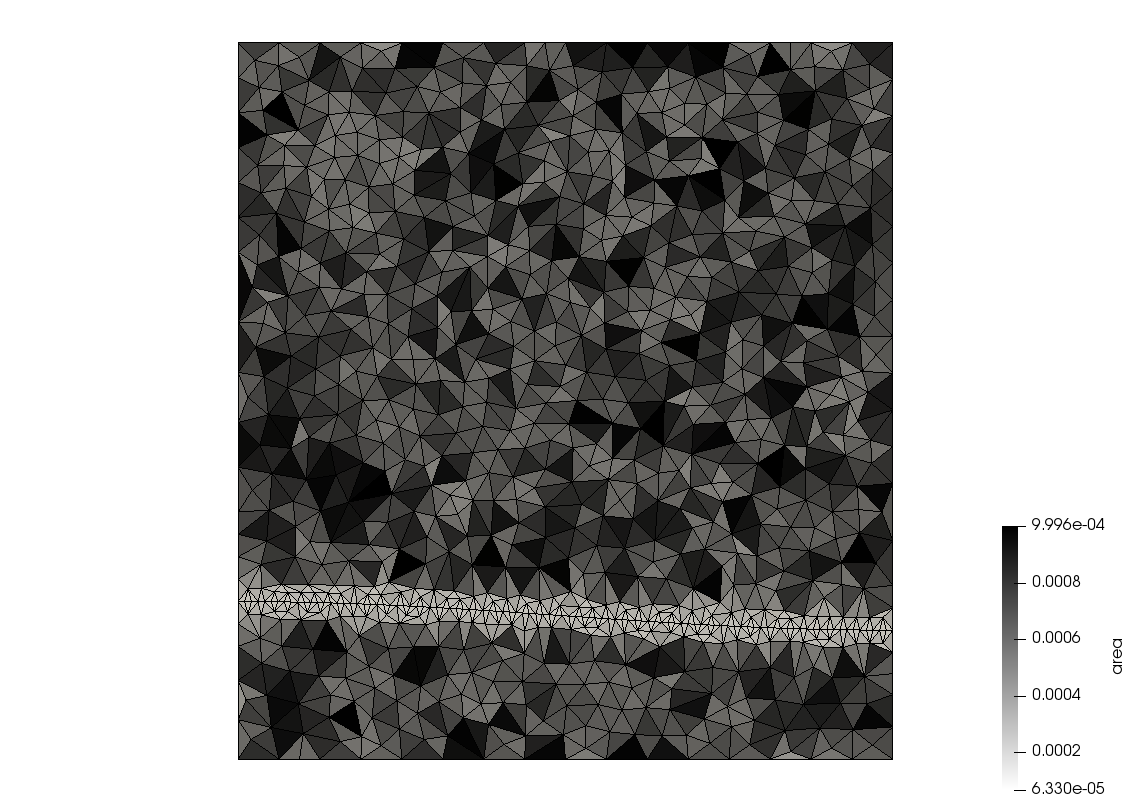
\includegraphics[width=5.5cm]{python_codes/fieldstone_95/init/area}\\
{\captionfont Interface counts 100 points, Triangle argument a=0.001, } 
\end{center}

The number of parameters one can vary is somewhat limited:
\begin{itemize}
\item the CFL number - default 0.25 (note that the time step is limited to 0.5);
\item the maximum area $a$ of triangles (passed as argument to Triangle) - default 0.001 for second order elements,
0.0005 of first order element;
\item the initial number of triangle vertices on the interface $np_{surf}$ - default 200;
\item the stretch factor controlling the addition of points $\gamma$ - default 1.5;
\item the type of element (element 1: MINI, element 2: Crouzeix-Raviart, element 3: Taylor-Hood)  
\end{itemize}

I also somewhat arbitrarily set the timestep to be limited to $\delta t_{\rm max}=0.25$. This allows for accurate 
measurements of the growth rate across all models. 
In the end we wish to plot the time evolution of the root mean square velocity and 
establish the time and amplitude of the first two peaks. We also wish to monitor volume/mass conservation.  

\newpage
%..........................................................
\subsubsection*{Isoviscous results - instantaneous results}.

\begin{center}
\begin{tabular}{|l|l|l|l|l|l|l|l|}
\hline
                & $a=0.002$     & $a=0.001$    & a=0.0008     & $a=0.0005$    & a=0.0004     & $a=0.0003$ & $a=0.0002$ \\ \hline
$np_{surf}$=150 &               &              &              & 1.852875e-04  & 1.852877e-04 & & \\ \hline
$np_{surf}$=200 & 1.852812e-04  & 1.852888e-04 & 1.852900e-04 & 1.852904e-04  & 1.852907e-04 & & \\ \hline
$np_{surf}$=250 &               &              &              & 1.852919e-04  & 1.852922e-04 & & \\ \hline
$np_{surf}$=300 &               &              &              & 1.852926e-04  & 1.852929e-04 & 1.852930e-04 & \\ \hline
$np_{surf}$=350 & 1.852838e-04  & 1.852916e-04 & 1.852924e-04 & 1.852932e-04  & 1.852933e-04 & 1.852936e-04 & \\ \hline
$np_{surf}$=400 & 1.852816e-04  & 1.852922e-04 & 1.852928e-04 & 1.852934e-04  & 1.852936e-04 & 1.852938e-04 & 1.852940e-04 \\ \hline
$np_{surf}$=450 & 1.852851e-04  & 1.852920e-04 & 1.852928e-04 & 1.852937e-04  & 1.852939e-04 & 1.852940e-04 & 1.852942e-04 \\ \hline
$np_{surf}$=500 & 1.852852e-04  & 1.852928e-04 & 1.852935e-04 & 1.852938e-04  & 1.852940e-04 & 1.852942e-04 & 1.852943e-04 \\ \hline
$np_{surf}$=550 &               &              &              & 1.852939e-04  & 1.852942e-04 & 1.852943e-04 & 1.852944e-04 \\ \hline
\end{tabular} \\
{\captionfont
Root mean square velocity $v_{rms}$ value for $t=0$. Crouzeix-Raviart element.}
\end{center}

%..........................................................
\subsubsection*{Isoviscous results - short term}

We now turn to the growth rate(s) which is measured in gnuplot as follows:

\begin{verbatim}
f(x)=a*exp(b*x)
fit f(x) 'benchmark_default.ascii' u 3:(($23-$21)) via a,b
\end{verbatim}

\begin{center}
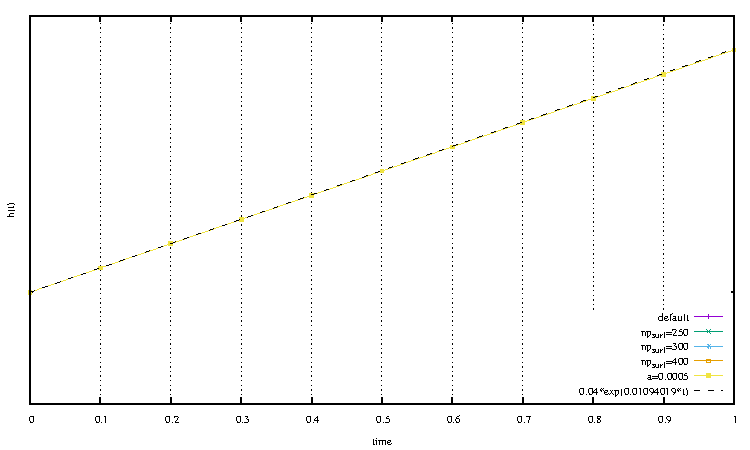
\includegraphics[width=5.5cm]{python_codes/fieldstone_95/results/growth_rate}
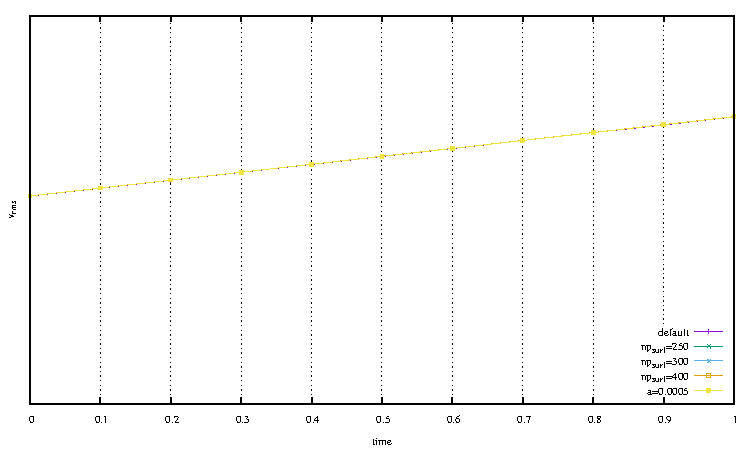
\includegraphics[width=5.5cm]{python_codes/fieldstone_95/results/growth_rate_vrms}
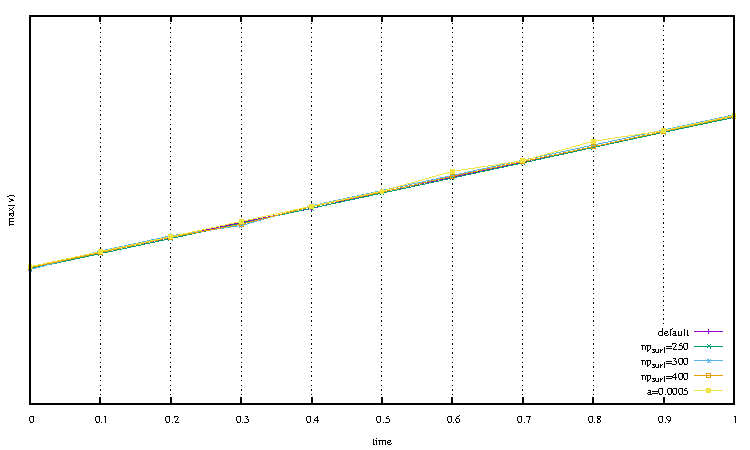
\includegraphics[width=5.5cm]{python_codes/fieldstone_95/results/growth_rate_maxv}
\end{center}


\begin{center}
\begin{tabular}{llll}
\hline
model    & $\gamma(h)$ & $\gamma(v_{rms})$ & $\gamma(\max(v))$ \\
\hline
\hline
default                 & 0.0108964 & 0.0110335& 0.0132341 \\
def. w/ $np_{surf}$=250 & 0.0108964 & 0.0110438& 0.0132409\\
def. w/ $np_{surf}$=300 & 0.0108964 & 0.0110449& 0.0134468\\
def. w/ $np_{surf}$=400 & 0.0108964 & 0.0110454& 0.0132651\\  
def. w/ $a=0.0005$      & 0.0108964 & 0.0110449& 0.0133781\\
\hline
\end{tabular}
\end{center}

%..........................................................
\subsubsection*{Isoviscous results - Long term evolution}

The script {\tt script\_run\_al} is designed to run for a long time (several days) 
and will lauch all 1+14 runs at the same time: 

\begin{tabular}{lccccc}
\hline
experiment &  CFL   &  $a$   & $np_{surf}$ & $\gamma$ & elt type \\
\hline
\hline
default    &  0.25  &  0.001 & 200         & 1.5      &  2        \\
\#1        &  '     &    '   & 250         & '        &  '        \\
\#2        &  '     &    '   & 300         & '        &  '        \\
\#3        &  '     &    '   & 350         & '        &  '        \\
\#4        &  '     &    '   & 400         & '        &  '        \\
\#5        &  '     &    '   & 500         & '        &  '        \\
\#6        &  '     &    '   & '           & 1.25     &  '        \\
\#7        &  '     & 0.0008 & '           & '        &  '        \\
\#8        &  '     & 0.0005 & '           & '        &  '        \\
\#9        &  '     &    '   & '           & '        &  3        \\
\#10       &  '     & 0.0005 & 400         & '        &  '        \\
\#11       &  0.1   &    '   & '           & '        &  '        \\
\#12       &  0.5   &    '   & '           & '        &  '        \\
\#13       &  0.75  &    '   & '           & '        &  '        \\
\#14       &  1     &    '   & '           & '        &  '        \\
\hline
\end{tabular}

Results are shown hereunder:

\begin{itemize}
\item minimum and maximum value of the velocity components $u$ and $v$:

\begin{center}
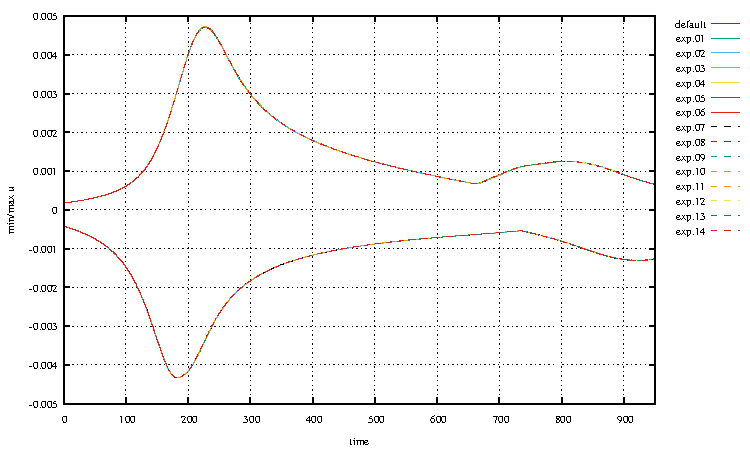
\includegraphics[width=7.5cm]{python_codes/fieldstone_95/results/u}
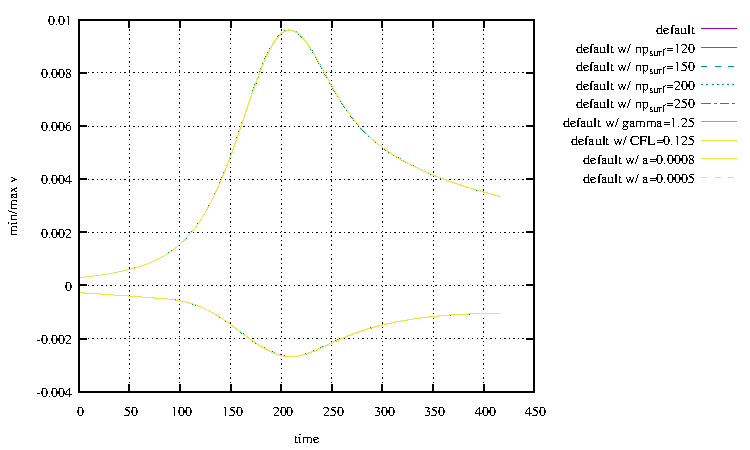
\includegraphics[width=7.5cm]{python_codes/fieldstone_95/results/v}\\
\end{center}

\item max($v$) for the first 10 seconds:

\begin{center}
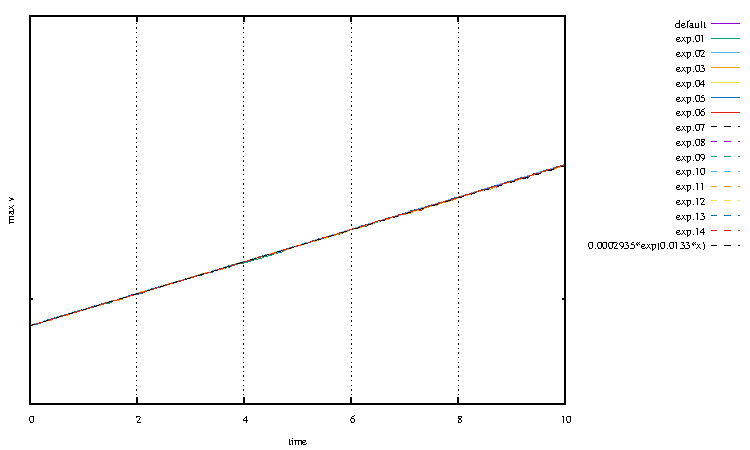
\includegraphics[width=7.5cm]{python_codes/fieldstone_95/results/v_start}
\end{center}

\item time step $\delta t$ value: 

\begin{center}
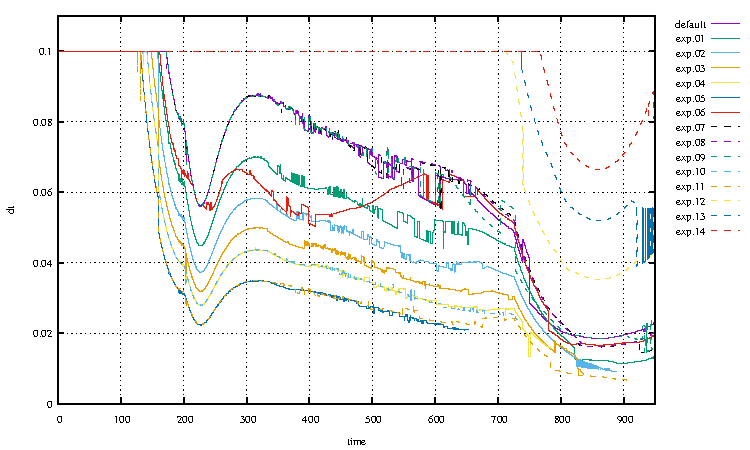
\includegraphics[width=7.5cm]{python_codes/fieldstone_95/results/dt}
\end{center}

\item volume of fluid 1 and 2 (relative change):

\begin{center}
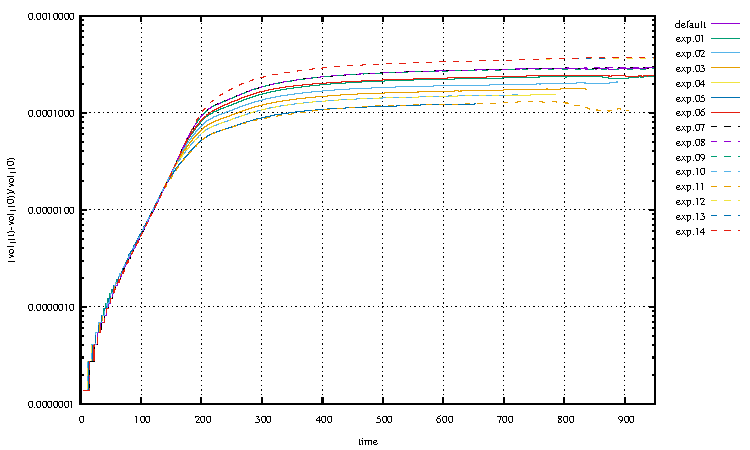
\includegraphics[width=7.5cm]{python_codes/fieldstone_95/results/vol1}
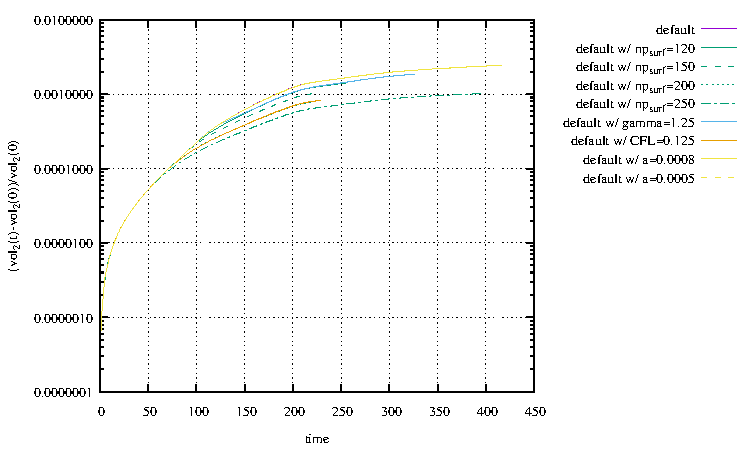
\includegraphics[width=7.5cm]{python_codes/fieldstone_95/results/vol2}
\end{center}

\item number of elements: 

\begin{center}
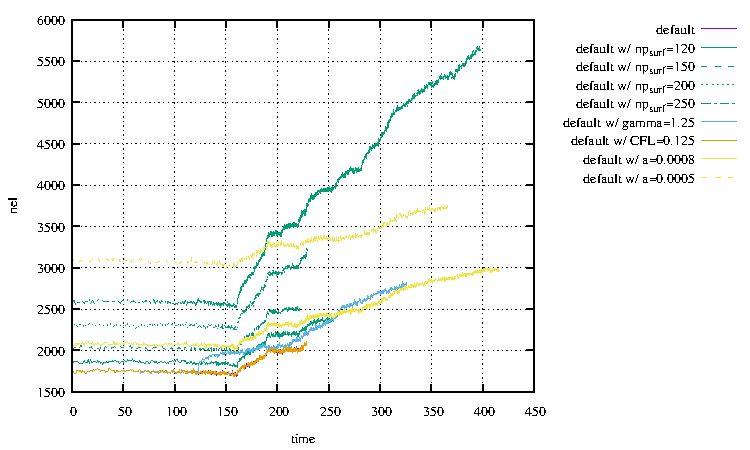
\includegraphics[width=7.5cm]{python_codes/fieldstone_95/results/nel}
\end{center}

\item velocity norm $|\vec\upnu|$
 
\begin{center}
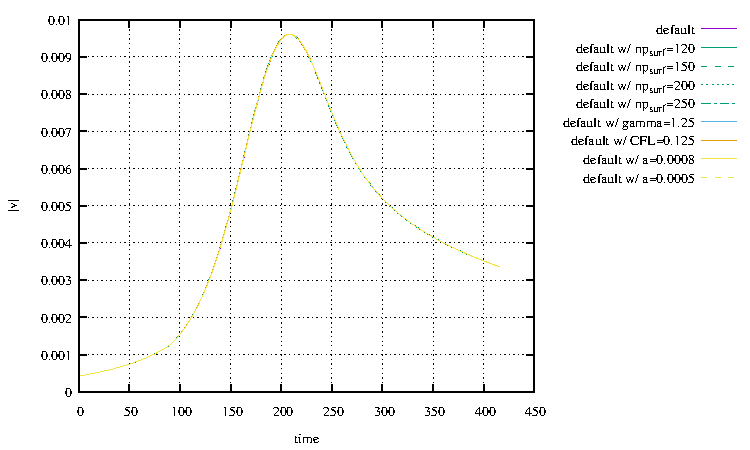
\includegraphics[width=7.5cm]{python_codes/fieldstone_95/results/vel}
\end{center}

\item The root mean square velocity

\begin{center}
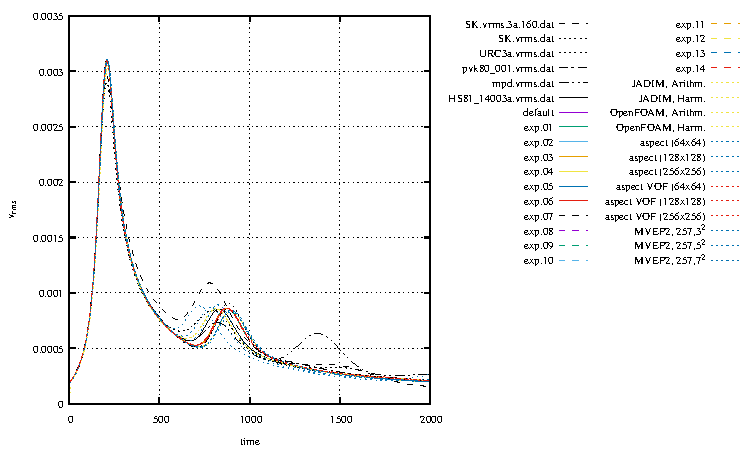
\includegraphics[width=7.5cm]{python_codes/fieldstone_95/results/vrms2000}
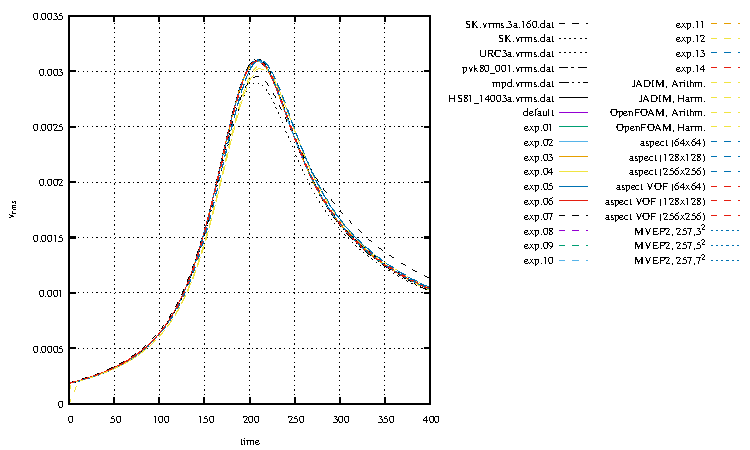
\includegraphics[width=7.5cm]{python_codes/fieldstone_95/results/vrms400}\\
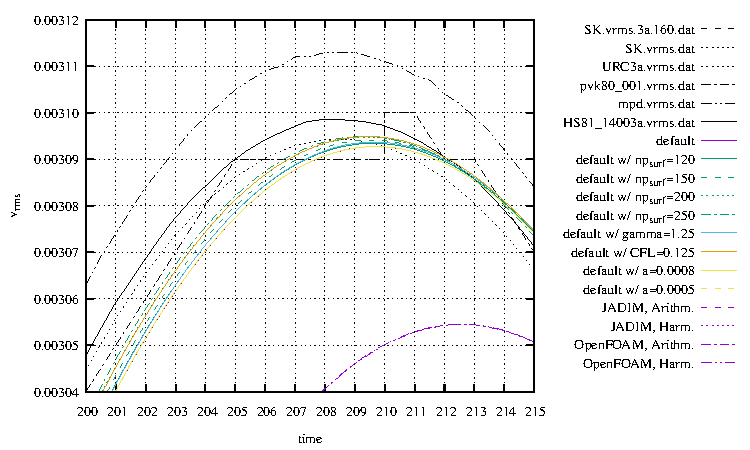
\includegraphics[width=7.5cm]{python_codes/fieldstone_95/results/vrms_peak1}
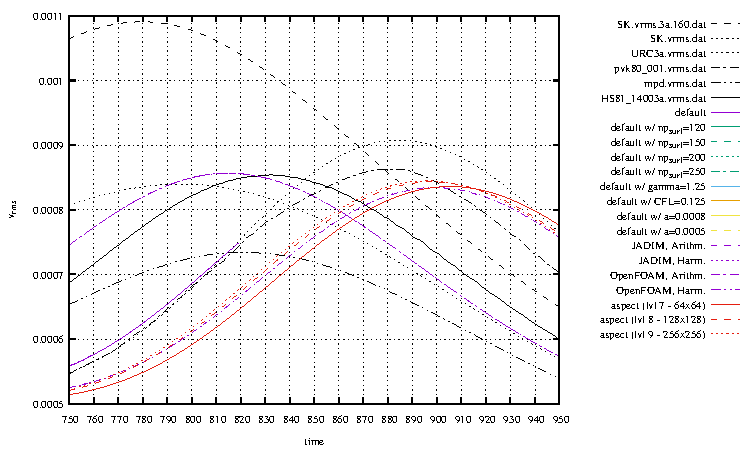
\includegraphics[width=7.5cm]{python_codes/fieldstone_95/results/vrms_peak2}\\
\end{center}

\item the number of points on the interface
and its length 

\begin{center}
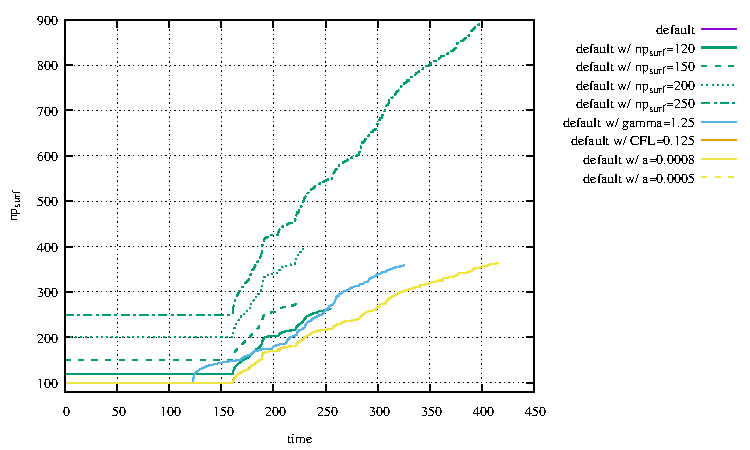
\includegraphics[width=5.5cm]{python_codes/fieldstone_95/results/np_surf}
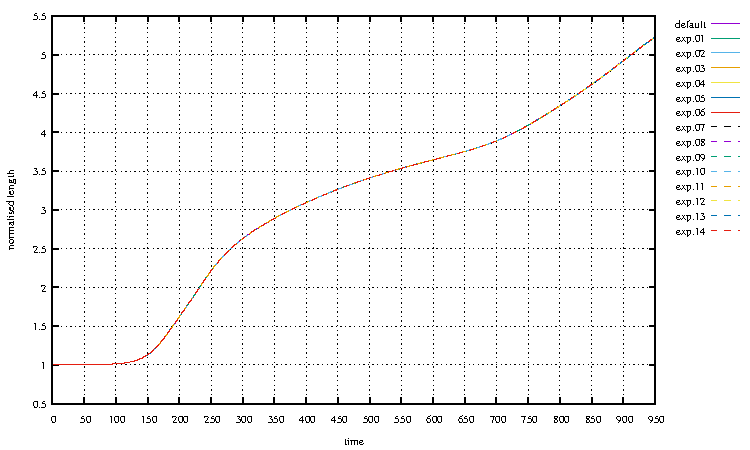
\includegraphics[width=5.5cm]{python_codes/fieldstone_95/results/length_interface}
\end{center}

\item the position of interseaction of the interface with the left and right boundaries: 

\begin{center}
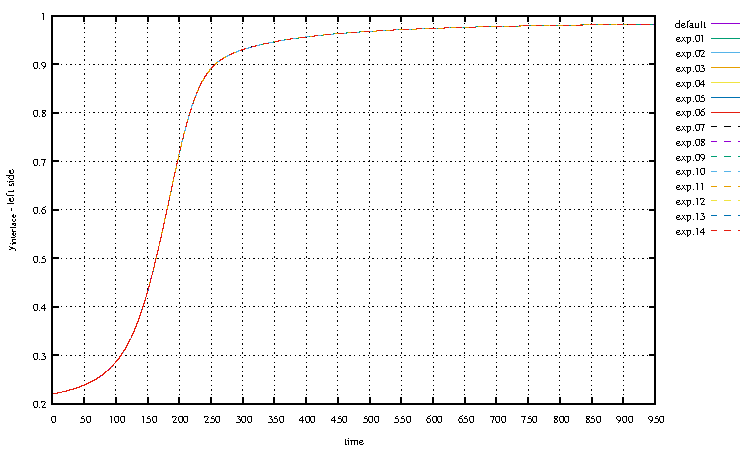
\includegraphics[width=5.5cm]{python_codes/fieldstone_95/results/left}
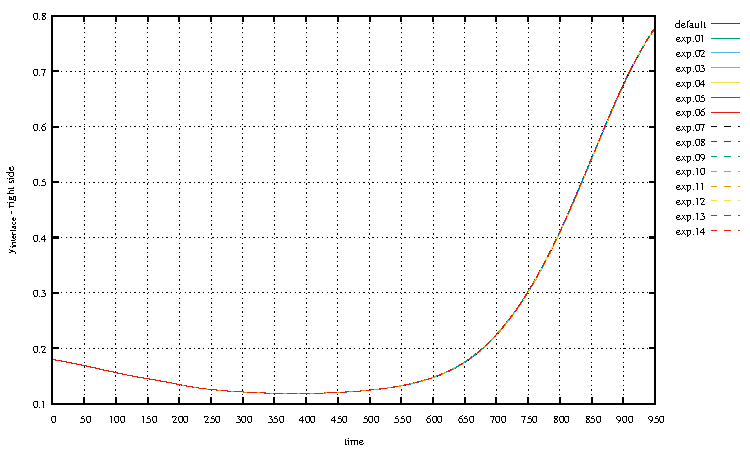
\includegraphics[width=5.5cm]{python_codes/fieldstone_95/results/right}
\end{center}

\end{itemize}




%\begin{center}
%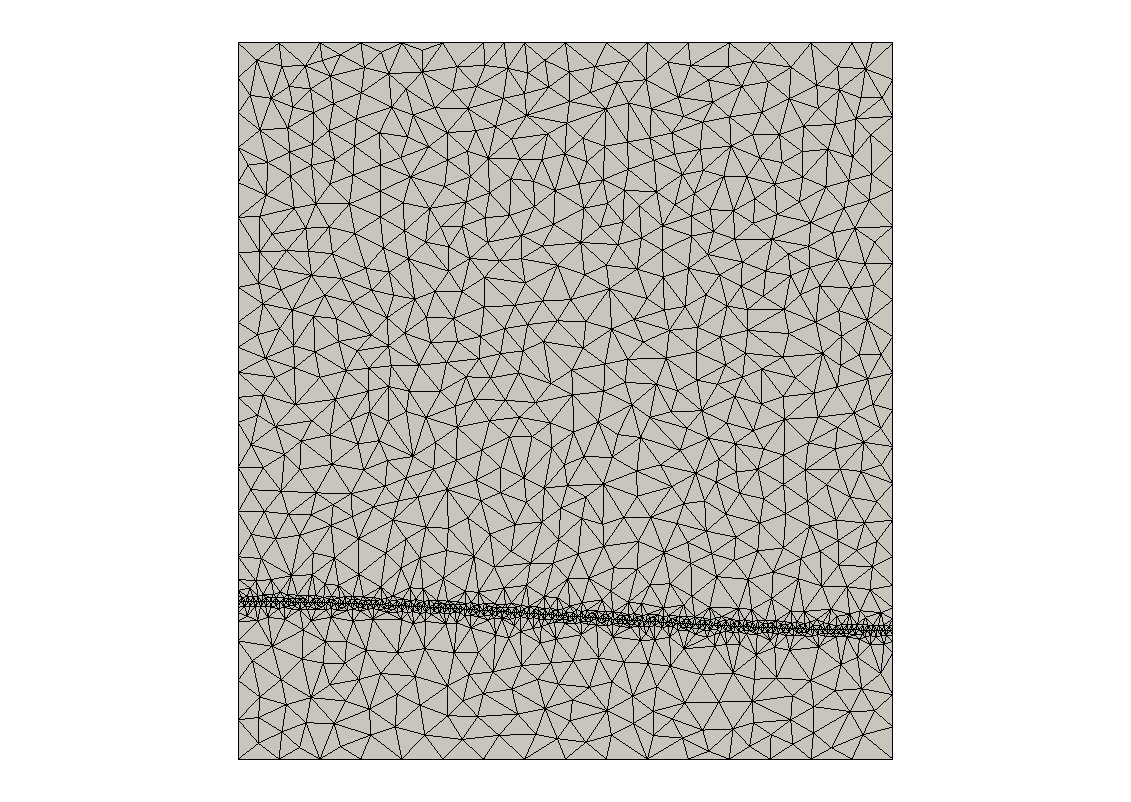
\includegraphics[width=5.5cm]{python_codes/fieldstone_95/results/npsurf250/grid0000.png}
%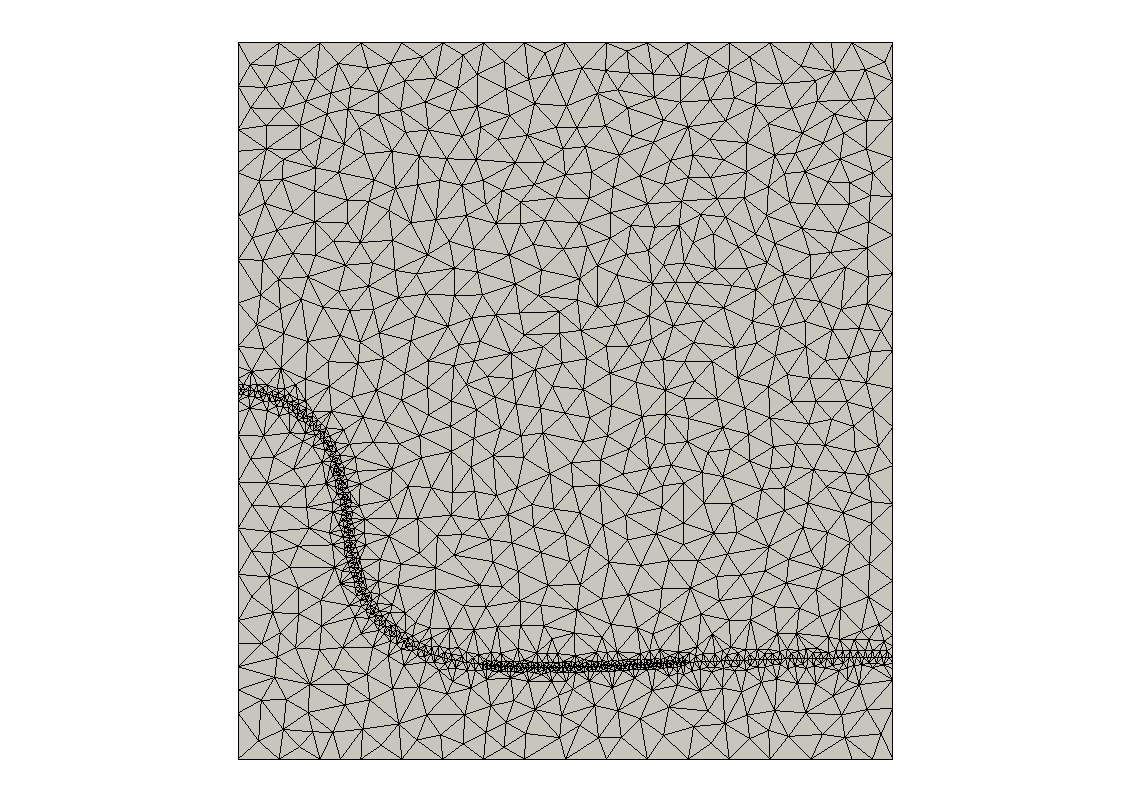
\includegraphics[width=5.5cm]{python_codes/fieldstone_95/results/npsurf250/grid0050.png}
%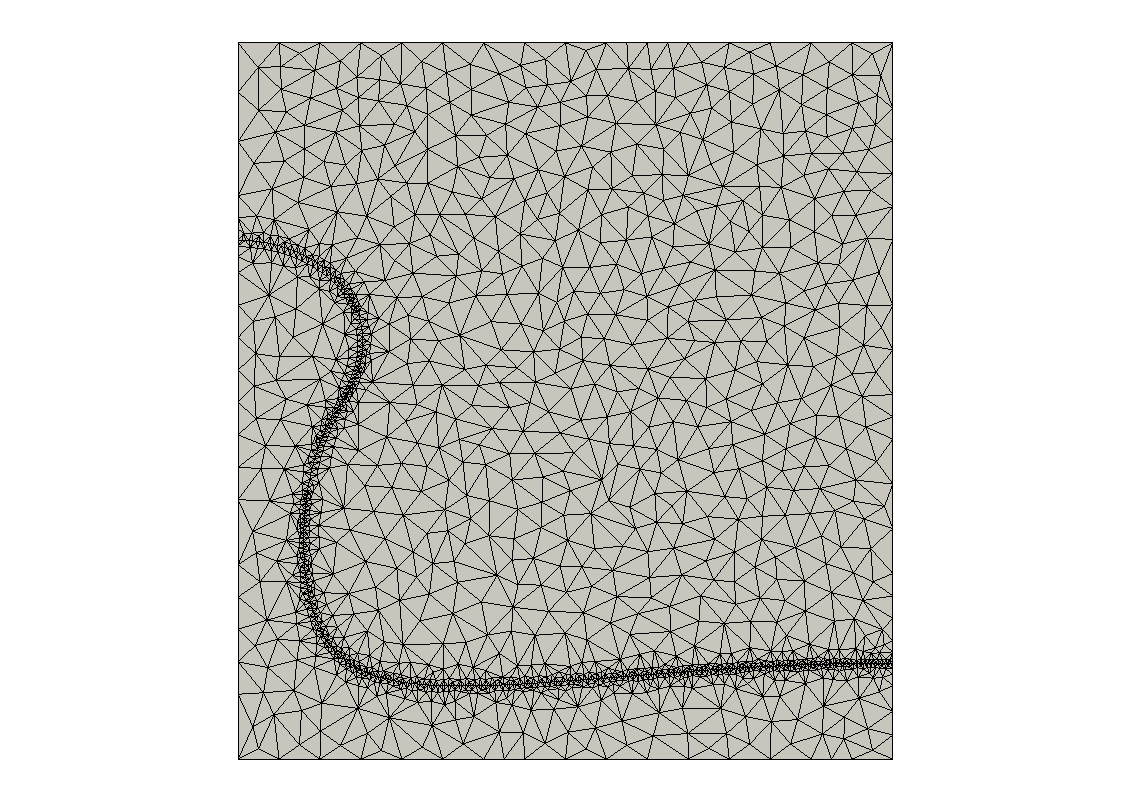
\includegraphics[width=5.5cm]{python_codes/fieldstone_95/results/npsurf250/grid0100.png}\\
%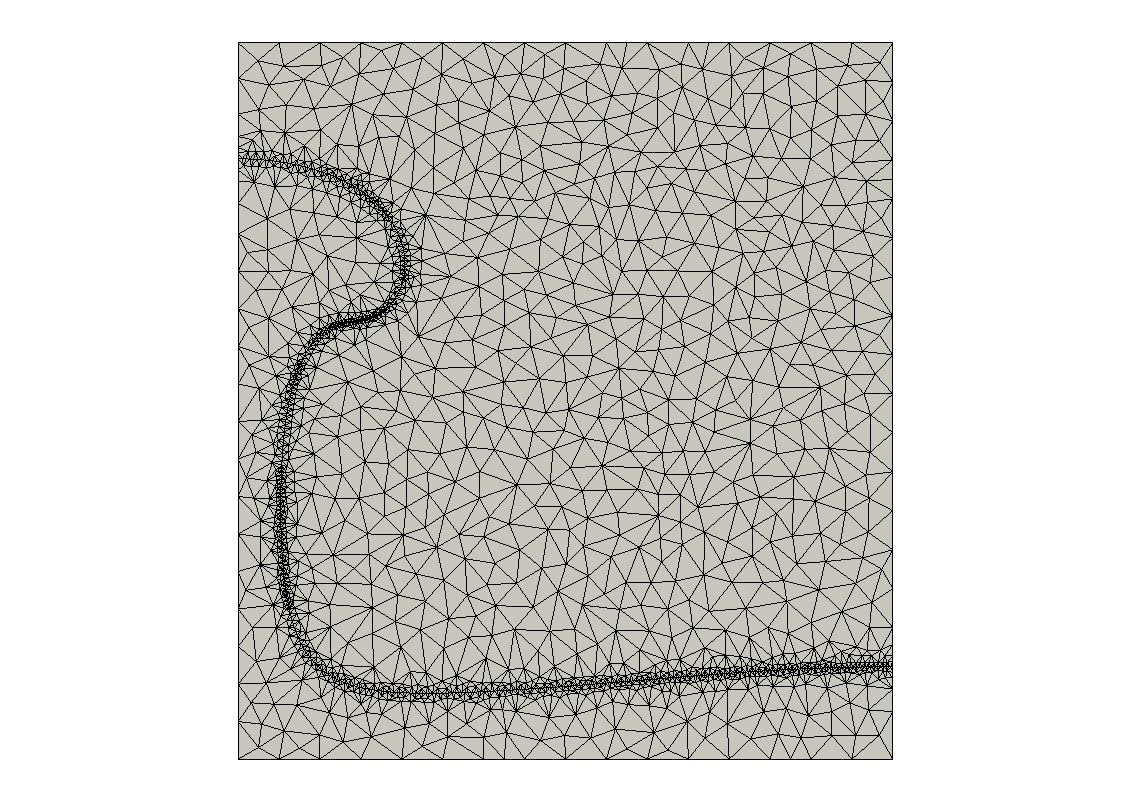
\includegraphics[width=5.5cm]{python_codes/fieldstone_95/results/npsurf250/grid0150.png}
%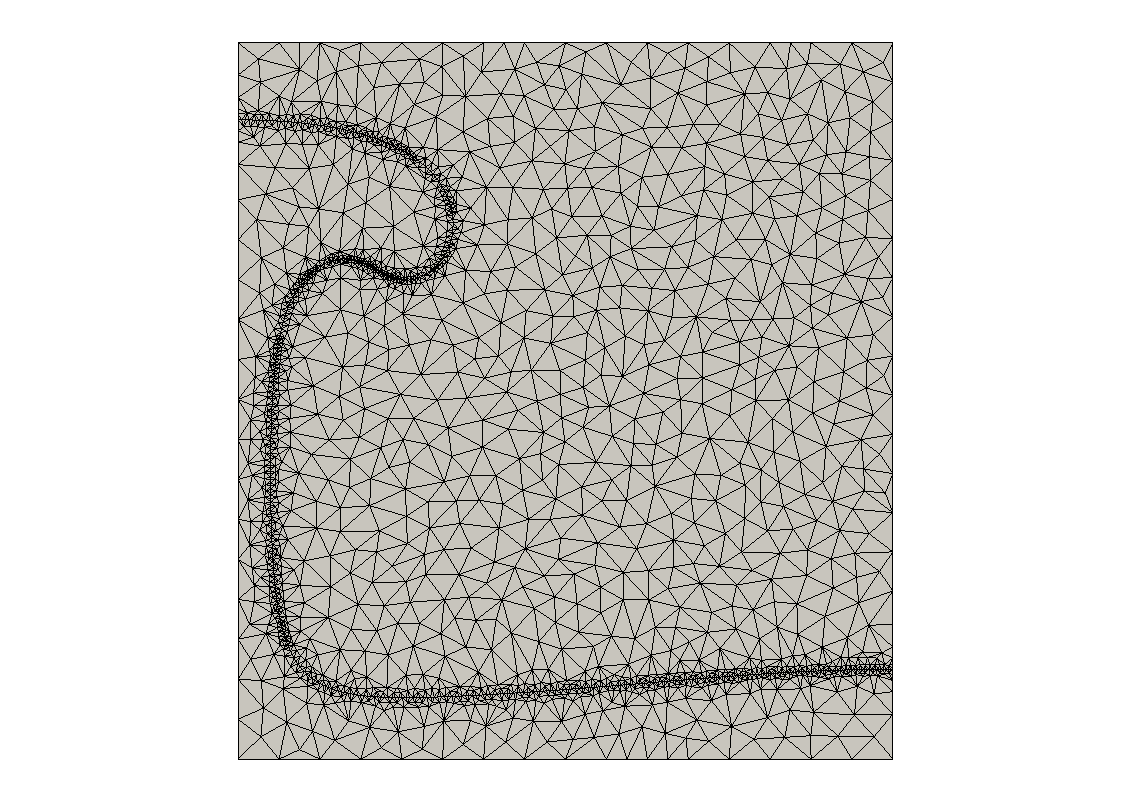
\includegraphics[width=5.5cm]{python_codes/fieldstone_95/results/npsurf250/grid0200.png}
%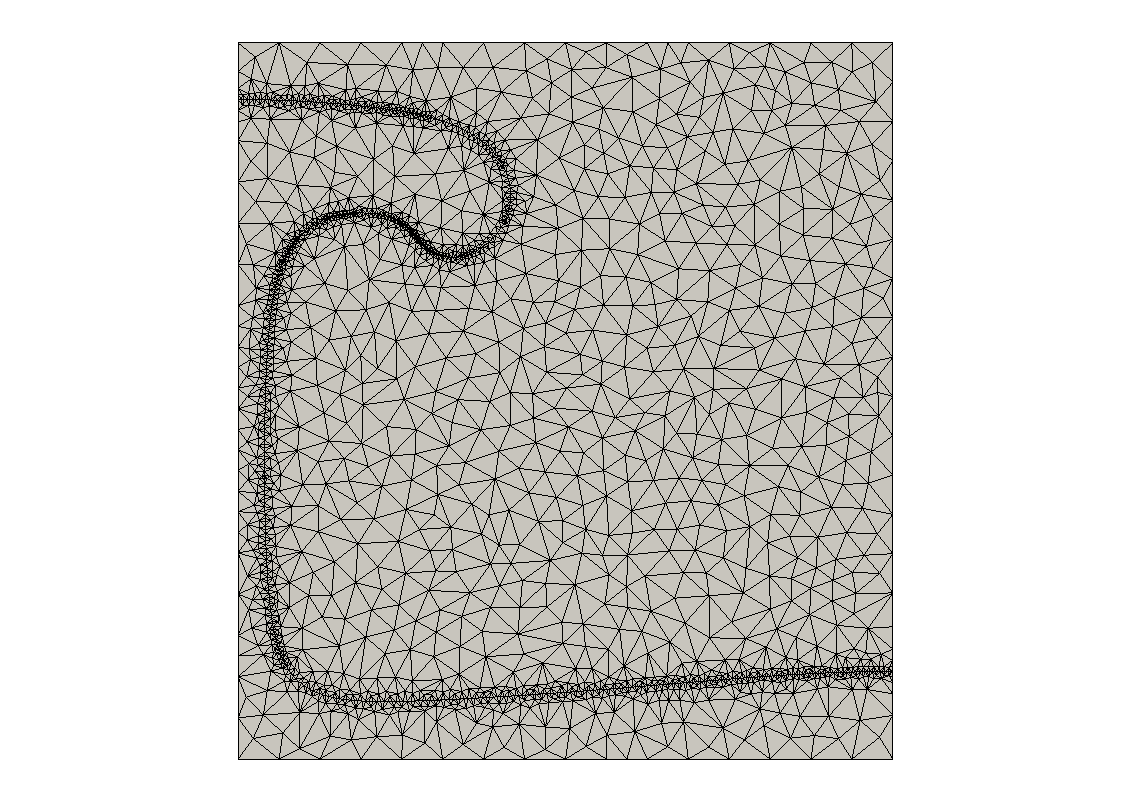
\includegraphics[width=5.5cm]{python_codes/fieldstone_95/results/npsurf250/grid0250.png}\\
%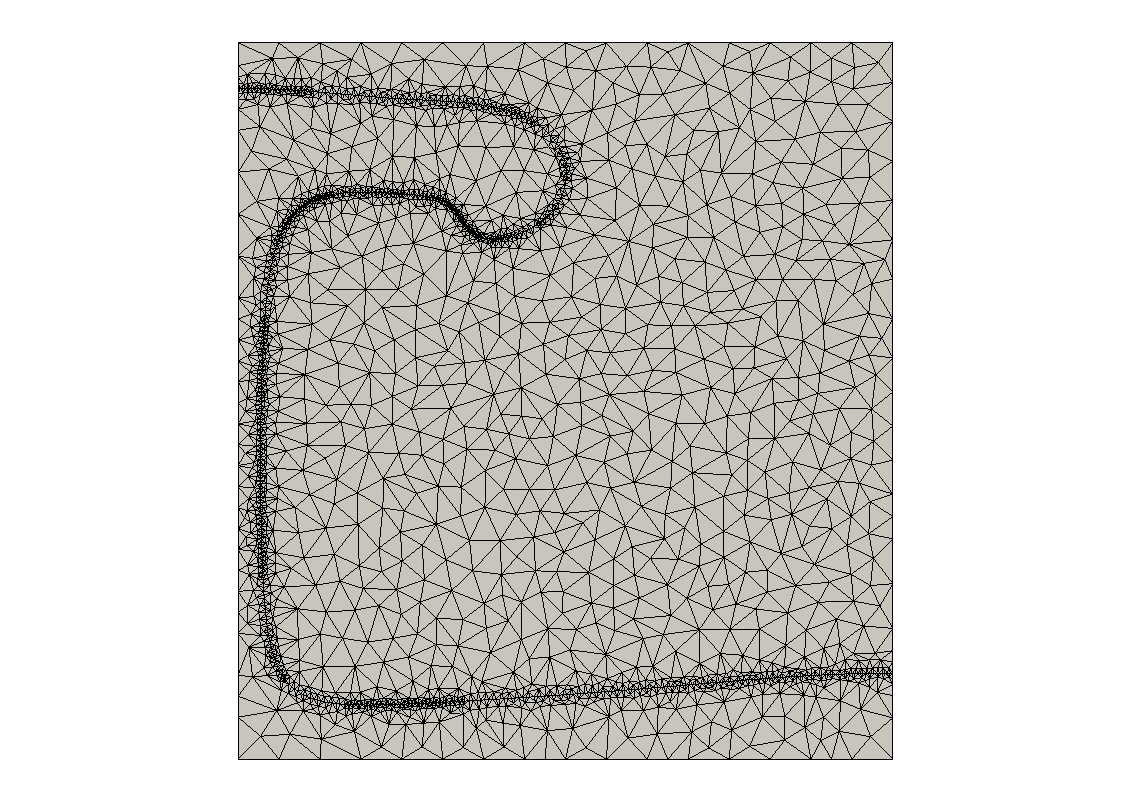
\includegraphics[width=5.5cm]{python_codes/fieldstone_95/results/npsurf250/grid0300.png}
%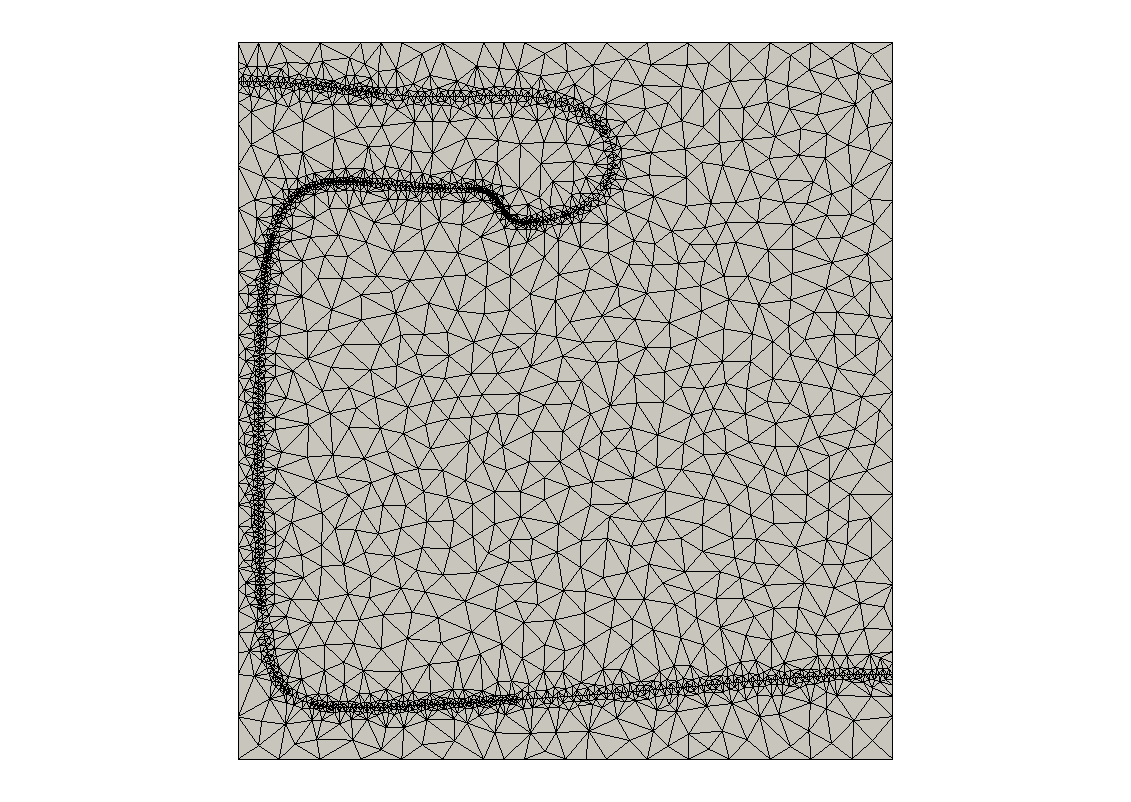
\includegraphics[width=5.5cm]{python_codes/fieldstone_95/results/npsurf250/grid0350.png}
%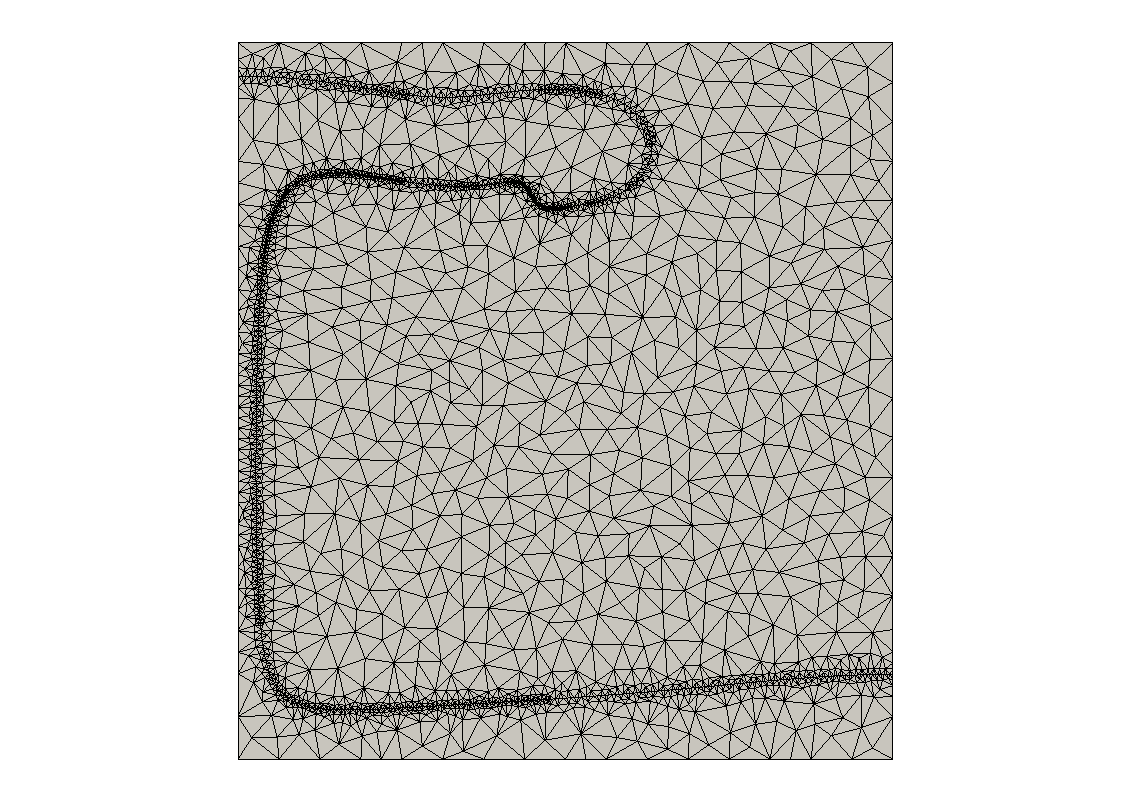
\includegraphics[width=5.5cm]{python_codes/fieldstone_95/results/npsurf250/grid0400.png}\\
%{\captionfont Cade default + npsurf=250, up to time = 400}
%\end{center}


I have also plotted the vrms against those of the original paper and those of Louis-Napoleon \etal \cite{logb20}
(with codes JADIM and OpenFOAM). 
The main parameter which seems to govern overal mass/volume conservation is the resolution of the interface. 

QUESTION: at the end of the first time step, when I write down the time associated with the measurements, should I write 0
or dt ?

QUESTION: does reduced density use change results ?

TODO: run until time=1500

TODO: viscosity ratio 10 and 100 cases

